\section{The Indicator (haylij) and Governor (kadhkhudah)}
\begin{mdframed}[backgroundcolor=cyan!5, rightmargin=1em, leftmargin=1em]
This  book is a bit of a nightmare to understand, the basic rules are jumbled in with definitions, delineations, and interpolated text across two chapters. In reading them I've often referred to Dykes \textsl{Carmen Astrologicum} and \textsl{Persian Nativities Vol. II} as well as Holden's \textsl{Abu'Ali Al-Khayyat: The Judgment of Nativities}, Hand's \textsl{Omar of Tiberias: Three Books on Nativities}, Deb Houldings Notes on Book III, Valens and Robert Zoller's DMA Course. As a result, the text in this section of the book has been extensively re-organized; an effort has been made to include references to the original chapter and line numbers.
\end{mdframed}

\subsection{Definitions}
Dorotheus describes some of the conditions that effect the ability of a planet to be effective (strong):
\begin{description}[style=multiline,leftmargin=7em]
\item[Eastern]\mn{1.4}a planet at least 15°\footnote{The 15° is a generalized value; Dorotheus gives 18° for \Mars, 19° for \Mercury\, and the same is usually assumed (see Dykes) for \Venus. Essentially, you want the planet to be visible, so the distance from the \Sun\, can vary depending on whether the planet is \textsl{superior} (\Saturn, \Jupiter, \Mars) or \textsl{inferior} (\Venus,\Mercury) and also based on the birth latitude. It is sometimes necessary to check actual \href{https://www.sunrise-and-sunset.com/en/sun}{sunrise-sunset times} for the day in question.} from the \Sun\, and rising ahead of it and visible
\item[Western ]\mn{1.5}a planet at least 15° from the \Sun\, and setting after it and visible
\item[Station] stationing direct or retrograde within 7 days before or after birth greatly strengthens the planet
\item[USB]\mn{1.6} a planet less than 15° from the \Sun\, is ``under the \Sun's'' rays or beams (usually referenced as USB); it is essentially invisible
\end{description}

Planets that are direct, eastern, and visible\footnote{see appendix \ref{appendix:visibility}:Visibility} are best at effecting what they signify. 

\subsection{Possible Indicator (haylaj or hyleg)}
Find the indicator first; begin with the \Sun\, in a day chart, the \Moon\, in a night chart \textsl{unless} the \Moon\, \mn{1.10} is New, Full, or making a phase\footnote{\textsl{ibid.}}, in which case she will be the indicator. 

If \mn{2.5} the chosen indicator does not receive an aspect from its term lord, triplicity lord\footnote{It is not clear whether the aspect must be from the first triplicity lord or anyone of the three. I suspect it must be the first triplicity ruler, the one coinciding with the chart sect.}, domicile lord, exaltation lord, or decan lord then it cannot be used as the indicator; \mn{2.2} check the other light, the Ascendant, the Lot of Fortune or the SAN in that order.

Once the indicator is identified, by default, its term lord or the lord in aspect, if it qualifies, becomes the governor (kadhkhudah or alcocoden).

\subsubsection{An Exception for the Lights}
If\mn{1.24} either light is in its own domicile (\Sun\, in \Leo, \Moon\, in \Cancer) and its term lord is in square or trine that light becomes the indicator and its term lord the governor\footnote{Presumably if this is true for both lights you would need to use the sect light or the best positioned light or possibly, the light whose term lord had the closest aspect.}

\subsubsection{The Sun}
In a day chart, the \Sun\, is the default indicator unless it is found to be in one of the following situations:
\vspace{-0.5em}
\begin{itemize}[topsep=0em,itemsep=0em]
\item \mn{1.15}in the 8th or 7th in a feminine sign, look to the \Moon
\item \mn{1.21}if cadent, look to the \Moon\, and if it is also cadent, look to the Ascendant
\end{itemize}

\subsubsection{The Moon}
\vspace{-0.5em}
In a day chart, if the \Sun\, does not qualify as the indicator, the \Moon\, will if she is found in one of the following situations:
\begin{itemize}[topsep=0em,itemsep=0em]
\item \mn{1.17}in the 10th or 11th in a feminine sign
\item \mn{1.18}in the 7th or 8th regardless of sign
\end{itemize}
If the \Moon\, is in the 12th or 9th, regardless of sign, \mn{1.21}look to the Ascendant\footnote{The preceding definitions imply that the \Moon\, must be above the horizon in a day chart and not cadent. As the \Sun\, has already been disqualified we are to move on to examining the Ascendant.}

In a night chart, the \Moon\, is the default indicator unless it is found to be in one of the following situations:
\begin{itemize}[topsep=0em,itemsep=0em]
\item \mn{1.19, 20}cadent or its lord is USB, in which case the \Sun\, is the indicator if it is in the 4th or 5th, \mn{1.21}otherwise look to the Ascendant
\end{itemize}

\subsubsection{The Ascendant}
If the \Sun\, or \Moon\, have been disqualified from being the indicator, or their lords have been disqualified from being the governor, examine the Ascendant degree. If its term lord is disqualified, examine the Ascendant's domicile lord and \mn{1.12} if it is USB \textsl{[or cadent?]}, examine its \textsl{[remaining lords: triplicity, exaltation, decan?]}\footnote{Dorotheus then tells us to see if the place \textsl{[sign?]} of this lord is masculine or feminine but he does not say if one or the other disqualifies the lord.}

If \mn{2.2} the Ascendant doesn't qualify check the Lot of Fortune, if it doesn't qualify, check the SAN.

\vspace{-0.5em}
\subsection{Possible Governor (kadhkhudah or alcocoden)}
If the lord of the indicator is found to be in one of the following situations  it is disqualified, move on to the next possible governor:

\begin{itemize}[topsep=0em, itemsep=0em]
\item \mn{1.18, 19} USB
\item \mn{1.11} cadent
\item \mn{2.23} does not aspect the terms the indicator occupies
\end{itemize}

If all the of the indicator's rulers are disqualified, move on to the next possible indicator.
\newpage
\subsection{Contradictory or unclear text re: the indicator and governor}
\begin{mdframed}[backgroundcolor=cyan!5, rightmargin=1em, leftmargin=1em]
This is essentially text that did not make sense in the context in which it appeared.
\end{mdframed}

\subsubsection{Indications from the Sun}
\begin{quote}
\mn{1.25}\textsl{Calculate if the \Sun\, is in the first degrees of \Aries\, and the lord of its [the \Sun's] term or house aspects it as this becomes the indicator.}
\end{quote}

\subsubsection{Indications from the Moon}
If \mn{1.7} the \Moon\, on the third day after the birth is in the term of:

\begin{itemize}[topsep=0em,itemsep=0em]
\item a benefic which is in a good place trine the \Moon\, while the \Moon\, is in an angular or succedent place ``then say that all of the nativity's condition is good''

\item either \mn{1.9} a benefic or malefic in a good place aspecting the \Moon, ``then it will be mediocre''

\item a \mn{1.8} malefic which is in an angle while Fortune is opposite the \Moon\, ``then say [that there is] no doubt that the nativity is bad''
\end{itemize}

\subsubsection{Indications from the Ascendant}
If \mn{1.22,23} the lord \textsl{[term or domicile? it's not clear]} of the Ascendant is disqualified from being governor ``then say [that there is] ruination in this nativity and that he [the native] will have no upbringing'' unless there is a benefic in the ascendant sign within 15° of the Ascendant.

\subsubsection{Other planets}
\begin{quote}
\mn{1.26}\textsl{ If \Mars\, and \Jupiter\, are in cardines or some of those that follow cardines or in the places which I mentioned above or in their houses or in their terms or in their exaltations or in their triplicities or in their portions, then it will be good as [those] planets will rule in the nativity which are in their house[s] or term[s] or image[s] [decans] or exaltation[s] or triplicities.}
\end{quote}

There has been some speculation that the above, coupled with the first chapter's opening paragraphs that describe various planet conditions, may mean any planet might act as the indicator (haylaj, hyleg) or that there is another technique used to identify a third planet that acts as the ``ruler of the nativity.'' Later authors do occasionally try to flesh out such a technique but to my knowledge there is no one agreed on, practical technique.

\newpage
\subsection{Longevity Example Chart 3.1.1}
\label{sec:longevity}
\vspace{0.5em}
\begin{mdframed}[backgroundcolor=cyan!5, rightmargin=1em, leftmargin=1em]
This particular chart is dated to February 26, 381 CE JC according to Ben Dykes (CAD p17) and so could not possibly have been included in Dorotheus' original manuscript as he lived in the 1st century, not the 4th. The other nine charts in the text have been dated between 12 and 44 CE. Dykes also believes the chart is based on the sidereal zodiac, although the oblique ascensions given agree with the values computed using the tropical zodiac for the year 381.

The method described, and referred to as \textsl{circumambulation} or \textsl{prorogation}, measures distances in zodiacal longitude and rate of motion in oblique ascensions, converting motion to time at the rate of 1° of OA = 1 year; the technique is the source of modern primary directions and secondary progressions the difference being that primary directions use 1° of right ascension as the rate of motion and measure of a year while secondary progressions use one day of the \Sun's motion in the ephemeris as the measure of one year.
\end{mdframed}

\vspace{-1em}
\begin{figure}[H]
\centering
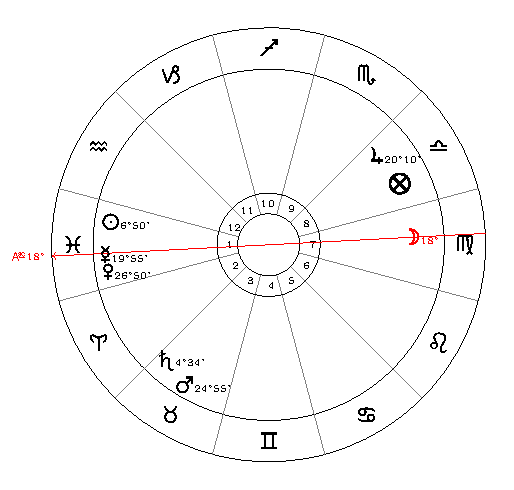
\includegraphics[width=0.8\textwidth]{charts/3_1_01}
\vspace{-1em}
\caption{Longevity Example Chart 3.1.01}
\end{figure}

Figure 3.1 is the chart of a person ``born in the ninety-sixth year of the years of Darinus [Diocletian] in the month of Mihr on the second day in one and a half equinoctial hours of daylight....in the 4th clime\footnote{The \Moon\, is missing from the chart in the text, assuming the Ascendant and \Sun\, degrees are roughly accurate, it should be around 18-19 \Virgo.}''. The author uses the chart to ``explain...the length of life and the number of years as \textsl{[he attempts]} [to compute it].''

\begin{quote}
\textsl{``I \mn{1.29} wanted to know the places of the haylaj among which he was born because they are five places, and none of the planets was in them except in the ascendant in which the \Sun\, was; and it is the best of places.''}
\end{quote}

The author has not spelled out ``the five places'' at this point, at a guess he is referring to the 1st, 7th, 11th, 10th, and 9th(?).  He says he chooses the 1st because the \Sun\, is there; that it is cadent by degree does not appear to matter, it is angular by whole sign. He then begins to direct the Ascendant (not the \Sun\, or its term lord) through the bounds.

\begin{quote}
\textsl{``I \mn{1.34-5}wanted to know in how many years the ascendant would conjoin with the rays of \Mars. I took the eighteen degrees of the ascendent and I found in the [tables for] my clime and the twelve parts [signs] [that] placed under it [was] three hundred and fifty-two [time] degrees and thirty seconds''}
\end{quote}

The Ascendant is at 18 \Pisces\, and \Mars\, is at 24 \Taurus\, 55, sending its sextile (\Sextile) ray to 24\Pisces 55. The author wants to know how long it will take for the degree imprinted by \Mars's sextile ray to rise up, by primary (diurnal) motion, to the Ascendant degree. He uses a technique commonly called \textsl{circumambulation} or \textsl{prorogation} that relies on the use of ``tables'', in this example, those for the 4th clime, to find the corresponding oblique ascension degrees for 18 \Pisces\, and 24 \Taurus\, 55. The 4th clime corresponds to Rhodes with a latitude of 36N\footnote{See \href{https://journals.sagepub.com/doi/10.1177/002182869302400105}{Verification of Parallax in Ptolemy's Hand Tables} by José Chabás and Anne Tihon }.

\begin{figure}[H]
\centering
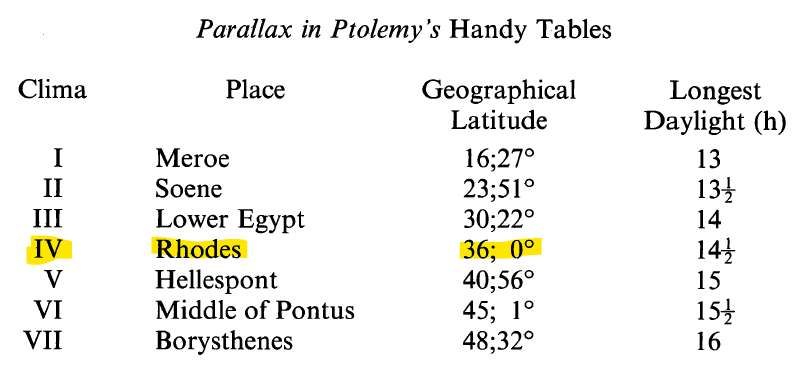
\includegraphics[width=0.7\textwidth]{diagrams/Ptolemy-climes}
\vspace{-0.5em}
\caption{Ptolemy's Climes}
\end{figure}

\begin{quote}
\textsl{``Then \mn{1.36-7} I took the twenty-four degrees and fifty minutes where \Mars\, cast its rays to \Pisces\, and I found the rising-times under this [to be] three hundred and fifty-six [time] degrees and forty-eight minutes''}
\end{quote}

Dykes gives the date of the chart as 381 CE, using \href{https://horoscopes.astro-seek.com/calculate-ascensional-rising-times/?latitude=100&narozeni_lat_custom_stupne=36&narozeni_lat_custom_minuty=0&narozeni_lat_custom_smer=0&narozeni_rok=381&aya=&oa=4&decimal=1}{Astro-Seek's Online Calculator} to calculate the oblique ascensions for custom latitude 36N in the year 381 CE the values for the two longitudes are within a few minutes of those given in the text:

\begin{quote}
\textsl{ ``[S]o I subtracted the three hundred and fifty-two [degrees] and thirty [minutes] which belong to the ascendent, and there were left four [time] degrees and eighteen minutes. And I said that the degrees of the ascendent would conjoin with the sextile rays of \Mars\, in four years and a fifth and a tenth of a year.''}
\end{quote}
From the Astro-seek tables (see Figure 3.3):

\begin{figure}[H]
\centering
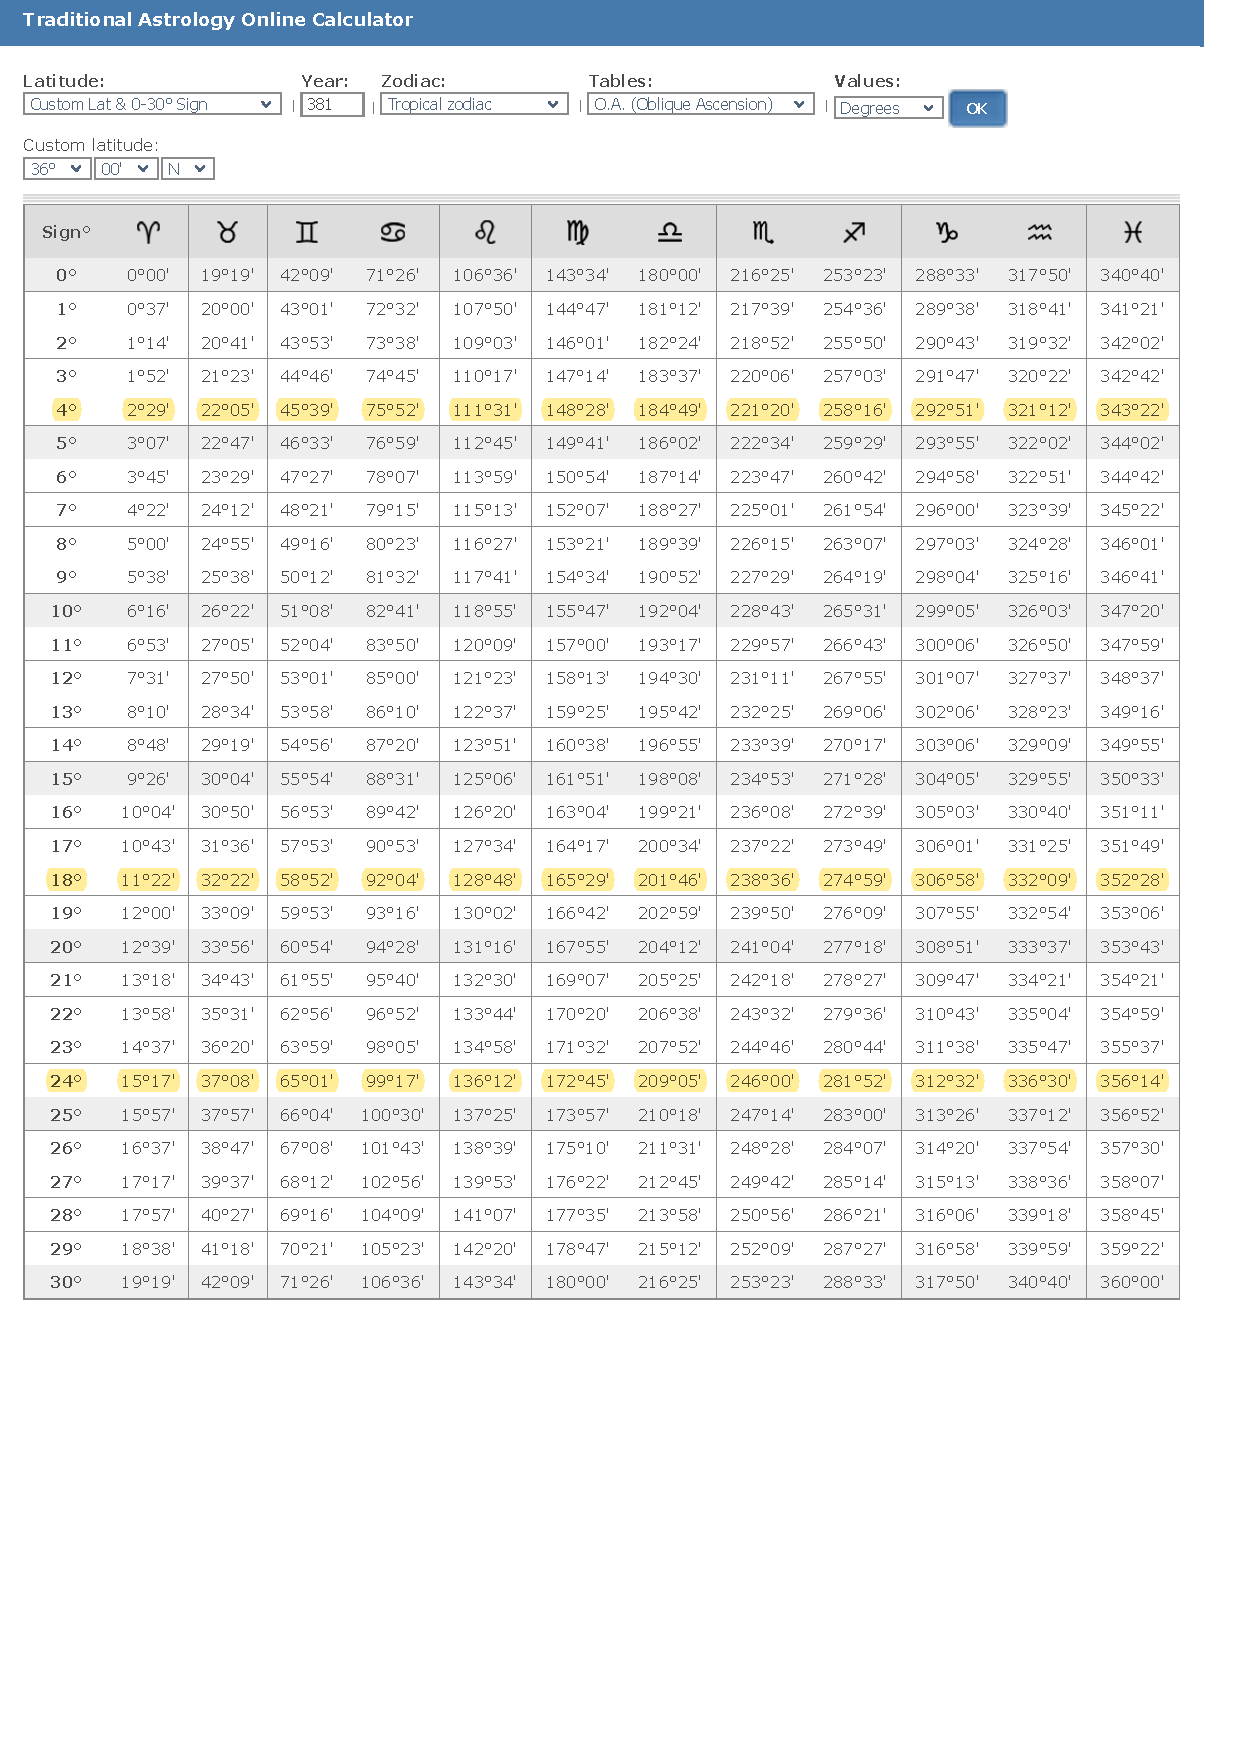
\includegraphics[width=0.9\textwidth]
	{diagrams/3.1.1-OA-Table }
\vspace{-8em}
\caption{OA table for Chart 3.1.1 calculated on Astro-seek}
\end{figure}

\begin{itemize}[topsep=0em,itemsep=0em]
\item[] \texttt{18\Pisces\,        352°28'    vs       352°30'}
\item[] \texttt{24\Pisces\,        356°52'    vs       356°48'}
\end{itemize}

The difference between 352°30' and 356°48' is 4°18' or 4 years, 3 months (18/60 = 0.3 x 12 = 3.6) and 18 (.6 x 30) days\footnote{Dykes explains the author's calculation as 18/60 = .3, 1/5 = .2 and 1/10 = .1 so 4 years plus 1/5 and 1/10 of a year (p.184 fn 34). It computes to the same 4 years + 365 x (1/5 + 1/10) = 4 years + 365 x 3/10 = 4 years 109.5 days or 4 years, 3 months, 18 days}.

\begin{quote}
\textsl{``Because \mn{1.38} \Venus\, [is] in this term, it dissolves the fear and misery that \Mars\, indicates and he will not die, but this misery will pass by him because whenever the rays of the benefics are found with the rays of the malefics, then the benefic dissolves whatever the malefic indicates; but if the malefic and its term cast rays without the benefics, then it will not be long before he dies.''}
\end{quote}

The sextile of \Mars\, falls at 24 \Pisces\, 55 in the terms of \Mars\, which run from 19-27° \Pisces. \Venus\, is sitting at 25 \Pisces\, 50 so she is in the same terms as the sextile ray and therefore removes its malice.

Next the author looked at when the Ascendant would contact 4 \Taurus\, 34, the degree the body of \Saturn\, was projecting itself to at the time of the birth. Using the same set of tables for the 4th clime, the oblique ascension of 4 \Taurus\, 34 was found to be 22° 21' (the Astro-seek table yields 22°23.8' if interpolation is used between 4 \Taurus\, and 5 \Taurus). Taking the difference between the Ascendant's OA of 352°30' and \Saturn's OA of 22°21' leaves 29°51' equating to 29 years, 1/2 + 1/4 + 1/10th of a year or 29 years 10 months and 10 days, the age at which the Ascendant will conjoin with \Saturn's degree.

\begin{quote}
\textsl{``Because \mn{1.50} the \Sun\, cast its rays from sextile to the first term of \Taurus\, where \Saturn\, was staying, the heat of the \Sun\, will drive away all the maleficence of \Saturn, and the harsh misery will pass him by, and he will not die.''}
\end{quote}

The first terms of \Taurus\, run from 0-7°; \Saturn\, projects to 4\Taurus\, and the \Sun, at 6\Pisces, throws his sextile to 6\Taurus\, so both \Saturn\, and the \Sun's ray fall in the same set of terms. The \Sun\, is apparently acting as a benefic here.

Next \mn{1.51-7} the author looked to see when the Ascendant would enter \Saturn's terms in \Taurus\, which begin at 22\Taurus, followed by it coming to the degree of the body of \Mars\, at 24\Taurus. He found the OA of \Mars\, in 24\Taurus\,55 to be 37°43' (the Astro-seek table gives 37°08' for 24\Taurus\, and 37°57' for 25\Taurus\, so 37° and 45' ((57-8) x 55/60)). He found the difference between this and the OA of the Ascendant to be 45°13' (37°43' + 360 - 352°30') or  45 years and 1/6 and 1/10 of a year or roughly 45 years 2 months and 19 days. 

\begin{quote}
\textsl{Because \mn{1.57} \Venus\, also cast its rays to this place from sextile, it will dissolve the maleficance of \Mars, and he will not die because of \Venus's aspect, and whatever of [its] rays it cast to this place, by means of them this misery will pass [him] by.
}
\end{quote}

In \Taurus, the terms of \Saturn\, run from 22-26°, \Venus, at 26\Pisces\,55 throws her sextile to 26\Taurus, within the same terms as \Mars\, and so protecting against any misery he might cause.

Neither  \mn{1.55-64} malefic throws its rays to the rest of \Taurus\, or to any degrees in \Gemini\, as both \Saturn\, and \Mars\, are in \Taurus\, and the Greeks did not recognize the semi-sextile (30°) as an aspect, as well, there is no mitigation between \Taurus\, and \Gemini, so he moves on to the sextile of \Saturn\, at 4\Cancer 34. He found the OA of the degree to be 76°20' (the Astro-seek tables yield 75°56') and the distance between the Ascendant OA to be 83°50' (76°20' + 360 - 352°30') or roughly 83 years 10 months and 4 days.
\begin{quote}
\textsl{Because the \Sun\, aspected from trine and cast [its] rays to this term in which are the rays of \Saturn, it will dissolve the misfortune this time, [but] he will die then when the rays of \Mars\, reach it [the ascendant].}
\end{quote}

The first degrees of \Cancer\, (0-6) are ruled by \Mars. \Saturn's sextile is at 4\Cancer\, the \Sun's trine falls at 6\Cancer\,50, within the same terms so he will ``dissolve the misfortune'' caused by \Saturn\, but when the Ascendant reaches the sextile of \Mars\, at 24\Cancer, in the terms of \Jupiter\, (19-25 \Cancer) he says  \Mars\, kills the person. \Venus's sextile falls to 26\Cancer, in the terms of \Saturn\, but \Jupiter's square falls at 20\Cancer\, in the same terms. Why does it not protect the person from death?  Most likely because \Jupiter\ occupies the 8th house and the person, by this time, is fairly old. The OA of 20\Cancer\, is 94°28' minutes, taking the distance from the OA of the Ascendant gives 101°48' or over 101 years old.

\subsection{Longevity Example Chart 3.2.1}
\vspace{0.5em}
\begin{mdframed}[backgroundcolor=cyan!5, rightmargin=1em, leftmargin=1em]
This chart example was most likely in Dorotheus' original text. Dykes, following Holden, dates it to October 2, 44 CE 8:15:01 AM JC using the tropical zodiac (CAD p87).  Unfortunately Dorotheus did not give the Oblique Ascensions or yearly values for the example so we can't easily test for the clime.
\end{mdframed}

\begin{figure}[H]
\centering
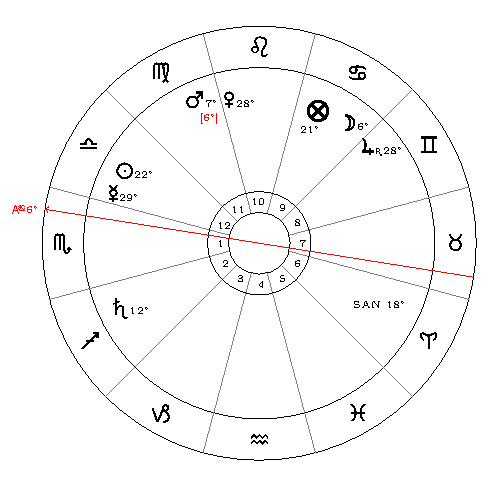
\includegraphics[width=0.8\textwidth]{charts/3_2_01}
\vspace{-1em}
\caption{Longevity Example Chart 3.2.01}
\end{figure}

\begin{quote}
\mn{2.19-22}\textsl{Because the nativity was diurnal, I looked in search of the haylaj at the \Sun, and found the \Sun\, cadent. I also looked at the \Moon, and I found it cadent. I found the lot of fortune and the fullness [of the \Moon] also in cadent[s]. There was nothing obvious from which the haylaj might be found except the ascendent.}
\end{quote}

The author began looking for the indicator by examining the \Sun\, as the chart is diurnal (\Sun\, above the horizon) but ended up rejecting it as a possible indicator (hyleg), along with the \Moon, \Fortune, and SAN, because they were all cadent. He ignores the fact that the 9th (holding Fortune and the \Moon) is a good house.

\begin{quote}
\mn{2.23}\textsl{The lord of the term of the ascendent, \Mars, was above the earth and near the East\footnote{Pingree appears to interpret this as \Mars\, being in the eastern hemisphere of the chart or nearer the the Ascendant, in the east but it is more apt to be a reference to the planet being \textsl{eastern} or rising before the \Sun.} and the four parts which have been mentioned and [in] the place of the good fortune aspecting the ascendent and casting [its] rays to that term in which the ascendent is, from above it, because it casts to the house and term together; if that casting were to the house only, it would not have this power. There is left of the term one degree that belongs to \Mars.}
\end{quote}

The Ascendant is at 6 \Scorpio, in the terms of \Mars\ (0-6 \Scorpio); making him the governor. \Mars\, more than qualifies as he is more than 15° from the \Sun\, and is rising before the \Sun\, (east), in a good place (11th), and sends his sextile ray to the ascendant. 

There seems to be a slight error in the text as we are told \Mars\, is at 7 \Virgo\, but that he casts his ray to his own terms, which end at 6 \Scorpio, with one degree of \Mars's terms in \Scorpio\, left. If that is true \Mars\, would need to be in, at the least, 6 \Virgo, and his sextile at 6 \Scorpio. 

The second last line of the paragraph implies that if the aspect falls to the house only, and not the term, \Mars\, would not ``have this power'' to be the governor. That is a limitation that was not mentioned elsewhere.

\begin{quote}
\mn{2.25-39}\textsl{So \Mars\, takes over the governorship of the prorogation and ray. Until this degree in its prorogation and its ray ends without the ray of any [other], \Mars\, indicates in this year injury from fire and disease. Even though \Mars\, is in a good place, it is necessary that it indicate like this. This misfortune is worse for him [the native] because the \Moon\, aspects it [\Mars]. If it were not that the \Sun\, stands between its ray and the ascendent and breaks the power of \Mars, it would be worse.}
\end{quote}

As the governor, \Mars\, manages the beginning of the native's life, which was prone to ``injury from fire and diseases'' (general significations of \Mars) regardless of the fact that \Mars\, occupies a good place (11th) and the risk is made worse by the fact that the \Moon\, (6 \Cancer) is \Sextile\Mars. Although the text does not mention it, she is also \Trine\ASC. The \Moon\, and the \ASC\, both signify the physical body, \Mars\, (injury) aspecting both increases the risk of physical harm.

We are then told that the \Sun\, ``stands between its ray and the ascendent and breaks the power of \Mars'', reducing the risk. The \Sun\, is at 22\Libra, he is in the 12th, averse to the 1st so he cannot cast a ray there, the only way the \Sun\, can break \Mars's ray is by his body since, as Deb Houlding points out, he is within 15° of the ascendent (DH p9) which means the \ASC\, would be combust, falling within the \Sun's light or glow, which in this case appears to protect the Ascendant from \Mars\, ray rather than harm the Ascendant itself\footnote{Evidence combustion can only harm planets?}.

\begin{quote}
\mn{2.30-32}\textsl{Then the prorogation of the ascendent comes to the term of \Venus\, till the eleventh degree. Because \Mars\, has left and \Venus\, has entered it is necessary to mix the power of these two together. Because of this the native will be blessed with love from his parents because both of these [planets] are in a good place, and moreover pain will reach him.}
\end{quote}

The ascendent will reach the terms of \Venus\, when it moves into 7\Scorpio. While the text says the power of \Mars\, and \Venus\, must be mixed because the terms of \Mars\, have been left, need to also keep in mind that \Mars\, will share the times by sextile with \Venus\, until the ray of another planet is met, which won't happen until the \ASC\, enters the terms of \Saturn\, (24-29\Scorpio) where \Venus\, throws her square to 28\Scorpio.

That the native will be loved by his parents is most likely indicated by \Venus\, (love) determined to parents by her opposition to the 4th (parents) and trine to \Saturn, ruler of the 4th. As well, \Venus\, is in the terms of \Mars\, herself, an indication she will show her significations when \Mars\, is ruling the times. As \Mars\, is still sharing in the times there continues to be a risk of bodily harm. 

\begin{quote}
\mn{2.33}\textsl{Then till the nineteenth degree is the prorogation of \Mercury, and in this period he will increase [his] learning and culture and the like.}
\end{quote}

The terms of \Mercury\, in \Scorpio\, run from 11° to 18°. During this period the native will be occupied with mercurial pursuits, namely ``learning and culture and the like.'' \Mars's is still sharing by sextile but his influence is not mentioned.

\begin{quote}
\mn{2.34}\textsl{The prorogation at puberty reaches \Jupiter, and it will indicate praise on account of [his] culture and good from [his] eloquence and the manifestation of [his] ways which are pleasing to people. Even though \Jupiter\, is retrograde in motion and does not aspect the \Moon\, and the ascendent, this will not decrease it because, whenever the planets are thus, their power is weakened and its gift is muddied. If \Jupiter\, were in a better place than this, it would increase the good.}
\end{quote}

The terms of \Jupiter\, in \Scorpio\, run from 19° to 23°, when the \ASC\, enters these degrees the things signified by \Jupiter\, will predominate; however, they will not be as good as they could be since \Jupiter\, is retrograde, does not directly aspect the \Moon\, or \ASC, and is in a bad place (8th). Again, there is no direct mention of \Mars\, influence even though he continues to share by sextile.

\begin{quote}
\mn{2.37-39}\textsl{The prorogation comes to \Saturn\, while \Venus\, casts [its] rays to the twenty-seventh degree of \Scorpio\, from quartile\footnote{\Venus's degree is given as 28\Leo\, in the chart description which still would throw a square to \Saturn's terms in \Scorpio.}, so that \Saturn\, and \Venus\, govern this prorogation together. \Saturn\, indicates his slowness in work and disease and distance from his land and grief and obstruction and difficulty, and this is worse because \Mars\, is elevated over \Saturn. If it were not that \Jupiter\, aspects \Saturn\, it would be worse.}
\end{quote}

When the Ascendant enters \Saturn's terms, which run from 24° to 29\Scorpio,  he will share the times with \Venus, who takes over from \Mars\, because her square falls at 28\Scorpio. The period will predominately be marked by ``slowness'' (\Saturn) , ``obstruction, difficulty'' (\Square), in ``work'' (\Saturn\, in 2nd of livelihood, \Venus\, in 10th of career), ``disease, grief'' (\Venus\, rules 12th) and ``distant from his land'' (\Saturn\, indicating absence?) All this is made worse by \Mars's square overcoming \Saturn\, in the radix and slightly lessened by \Jupiter's opposition to \Saturn.

\begin{quote}
\mn{2.40}\textsl{Because of the place of \Saturn\, his mother will die in this period...}
\end{quote}

This is a little odd at first until you realize that (a) \Venus\, rules the mother in a day chart, (b) the Lot of the Mother falls at 14\Virgo\footnote{The Lot of the Mother is given in 1.14 as being calculated from \Venus\, to the \Moon\, projected from the Ascendant (the text actually says to subtract the difference from the Ascendant ``by day'' but this is likely an error, the majority of other sources says to add it.)}, in the 8th from the 4th (parents), and (c) it is square \Saturn\, whose place in the 2nd also signifies death by his opposition to the 8th. As well, in 1.15 we are told that the parent who will die first is the one whose lot is in the same place as a malefic or is opposed or square to a malefic. The Lot of the Mother is in \Virgo, with \Mars, and is square \Saturn. And, while the Lot of the Father at 26\Sagittarius\footnote{The Lot of the Father is given in 1.13 as being calculated from the \Sun\, to \Saturn\, and projected from the Ascendant.} is in a similar position (in the same sign as the malefic \Saturn\, and square the malefic \Mars) the aspect between \Saturn\, and the Lot of the Mother is stronger (2°) than the one between the Lot of the Father and \Mars\, (21°), the Lot of the Mother is actually in the sign of the parent's death, \Venus, the main significator of the mother in a day chart has a share of the times, the \Sun, main significator of the father in a day chart, does not.

\begin{quote}
\textsl{... but he will acquire goods because \Saturn\, indicates these, and he will marry a wife with a dowry, and [a child] will be born to him who will live a short while and die in the third year; his enjoyment of women and children will be from \Venus, but his lament and the death of his child will be from \Saturn.}
\end{quote}

The acquisition of a wife is shown by \Venus\, indicating a ``wife'' by her nature and by being ruler of the 7th (spouse, marriage). Goods and a dowry, by \Saturn\, (property) in opposition to the 8th (wife's money). Children are shown by \Jupiter\, ruling the 5th (children). The child's life and death is shown by \Jupiter\, in the 8th (death), where it is retrograde and acting as an accidental malefic (a benefic connected with bad places or severly injured). As well, \Venus\ rules the 12th (8th from the 5th) and is sextile \Jupiter.   Zoller taught that an accidental malefic was most likely to give a benefit according to its nature and then, if retrograde, take it away. 

The ``three years'' probably comes from the degrees 27 (\Venus's position) minus 24 (beginning of \Saturn's term) although it seems to be a bit of a fudge as he originally gave \Venus's degree as 28 and normally oblique ascension values, not longitudinal degrees, would be used to time the event.

\begin{quote}
\mn{2.41-43}\textsl{Then the prorogation arrives at \Sagittarius, the first term, which is the house of \Jupiter\, and its term. Because \Jupiter\, makes this place its house and its term, it governs the prorogation alone without any [other] of the planets [and] it increases its power. It indicates for the native leadership and honor among groups of men, and his elevation among them.}
\end{quote}

This adds another wrinkle to ``who'' actually governs the times. Normally it would be the new term lord \textsl{and} the planet ruling by ray (in this case \Venus) but here we are told that because \Jupiter\, is both the domicile ruler and the term lord he ``governs the prorogation alone.''

\begin{quote}
\mn{2.44}\textsl{Because \Saturn\, is in the twelfth degree, it indicates the last day of his life, and he will live after the twelfth degree for forty-eight nights because \Saturn\, is in the beginning of the degree [at 12°8'].}
\end{quote}

The person will die when the Ascendant meets the body of \Saturn\, at 12\Sagittarius. The 48 nights comes from 8 minutes /60 x 365 days. While \Saturn\, is in the terms of \Jupiter\, (0-11\Sagittarius) \Jupiter, in the 8th of death, has been shown to be an accidental malefic who does not throw a ray to the same terms and neither does \Venus\, (at 28\Leo), the other benefic.

\subsection{Additional Advice on Prorogations}
The author advises us to look not only at the prorogation of the Ascendant but also at the prorogation of the \Moon:
\begin{quote}
\mn{1.66}\textsl{...because the conjunction of the \Moon's degree with the malefics indicates misery, especially if with this the benefics do not aspect as, if they do aspect, they dissolve misery and death}
\end{quote}

\noindent As well we are told...
\begin{quote}
\mn{1.67-68}\textsl{It is necessary for you to look at the transit of the planets and the revolution of years\footnote{This most likely refers to the practice of \textsl{profecting the chart} (turning the chart at the rate of one sign per year) which is described in Book IV.}; in these sometimes it makes him miserable and spoils [his] life, but we do not find this peculiarity in everyone [of the books]. I sought for this in a long period of years and I suffered every misery so that I might write it down.}
\end{quote}
\noindent And that we need to pay special attention to a planet's latitude:
\begin{quote}
\mn{1.69-71}\textsl{Look at the casting of the rays in latitude also because sometimes a planet is aspecting from opposition, and if you calculate it in latitude and you find one (planet) in the south, the other in the north, then this is not in opposition and also does not cast [its] rays, which according to this indicates misery. Also if you find both the \Sun\, and the \Moon\, in the sixth or the eighth or the twelfth and the malefics aspect [them], then they indicate death when their degrees conjoin with malefics. But if they are in a bad place but are not injured, and you find the malefics casting [their] rays close to their degrees, then the misery which would be will pass by, and he will not die of it.}
\end{quote}

The rays of planets at different \textsl{latitudes} reach the various longitudinal degrees at different times depending on how far they are to the north or south of the ecliptic, which can completely alter the timing and or even completion of aspects i.e. planets that look as though they are nearing an aspect may actually be well past it.

\noindent And lastly, we have a loose summary of the technique:
\begin{quote}
\mn{2.45}\textsl{If you want to know how each planet increases the nativity and how it diminishes it, then look at the transit of the planets and which aspects the haylaj from right or left, and [look] at the term of the ascendent and at the lord of the ascendent's term and the planets which are in it.}
\end{quote}
The above implies we should always direct the Ascendant, whether it is the indicator (haylaj, hyleg) or not.

\begin{quote}
\mn{2.46-48}\textsl{Consider well the rays, whether of benefics or of malefics or mixed, because if the rays are of malefics without benefics' then it is bad. See which [planet] casts [its] rays in aspect or in being with it [the haylaj?], and in how many degrees of rising-times in the clime in which you are it will arrive at the prorogation. Consider the planet which casts [its] rays to the planet which aspects it [the haylaj?] or [is] with it and the lord of the prorogation; then mix them together in proportion to their maleficence and their beneficence and their power in the places and the planets' aspect of them and their portions and their terms and their houses, and judge in accordance with how you find them.}
\end{quote}

\begin{quote}
\textsl{The third book of the books of Dorotheus is finished. Praise to God---He alone deserves praise and merits it.}
\end{quote}
